\section{Durchführung}
\label{sec:Durchführung}


\subsection{Aufbau}

Für alle Versuchsteile wird ein Generator mit variablem Schwingungsmuster verwendet.
Ein Stromkreis mit Spule Kondensator und variablem Ohmschen Widerstand wird an den Generator angeschlossen.
Die Messungen werden mit einem Oszilloskop mit Hochohmigem Tastkopf vorgenommen. 

\subsection{Messung}

\begin{figure*}[h!]
    \centering
    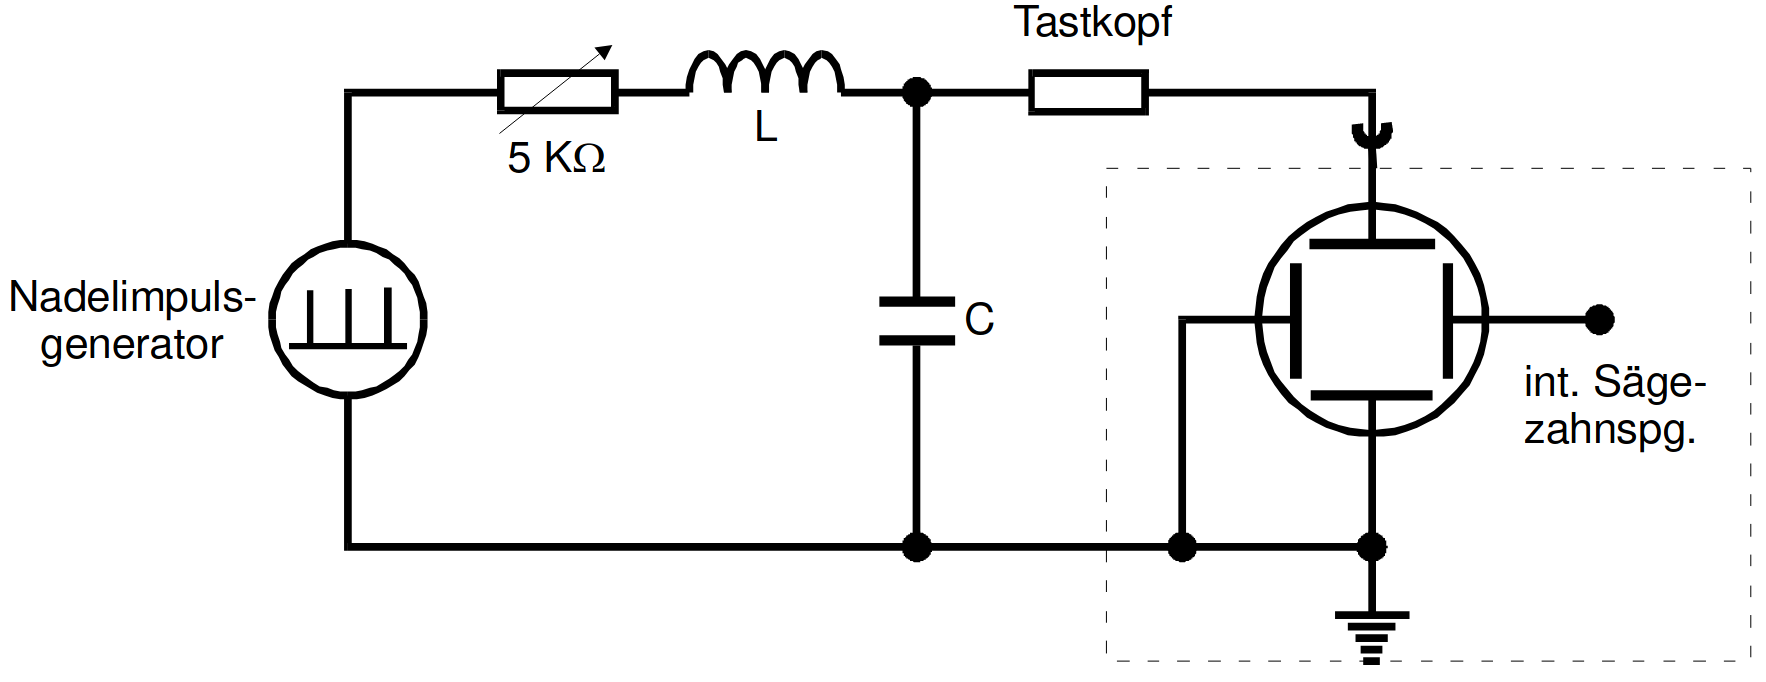
\includegraphics[width=\linewidth]{build/Kreis1.png}
    \caption{Schematischer Aufbau des ersten Versuchteils.\cite{V354}}
    \label{fig:Aufbau1}
\end{figure*}

Im ersten Aufgabenteil wird der Effektive Dämpfungswiderstand des Schwingkreises ermittelt. Dazu wird eine Rechteckspannung an den Stromkreis angeschlossen.
Die Spannungsfrequenz wird so gewählt, dass sich die Schwinungsamplitude etwa um den Faktor 3 verringert. 
Der Anzeigebereich des Oszilloskops wird so gewählt, dass die volle Schwingungsdauer auf dem Bildschirm abgebildet werden kann.
Es werden Messwertpaare der Form $(t, U_C)$ aufgezeichnet. Es werden Spannungen für die obere als auch die untere Einhüllende in zwei seperaten Tabellen aufgenommen.\\
\\
Im zweiten Aufgabenteil wir der Widerstand $R_{\text{ap}}$ ermittelt. Der Widerstand aus dem ersten Aufgabenteil wird durch einen kontinuierlich einstellbaren Widerstand ausgetauscht.
Zu Beginn wird $R = \SI{5}{\kilo\ohm}$ gesetzt. Der Schwingkreis zeigt nun reines Relaxationsverhalten. 
Der Widerstand wird nun so lange abgesenkt bis wieder oszillatorisches Verhalten erkennbar wird. Nun wird
der Widerstand feinjustiert, so dass die Entladekurve am schnellsten ohne überschwingen gegen Null geht.
\\
\\
\begin{figure*}[h!]
    \centering
    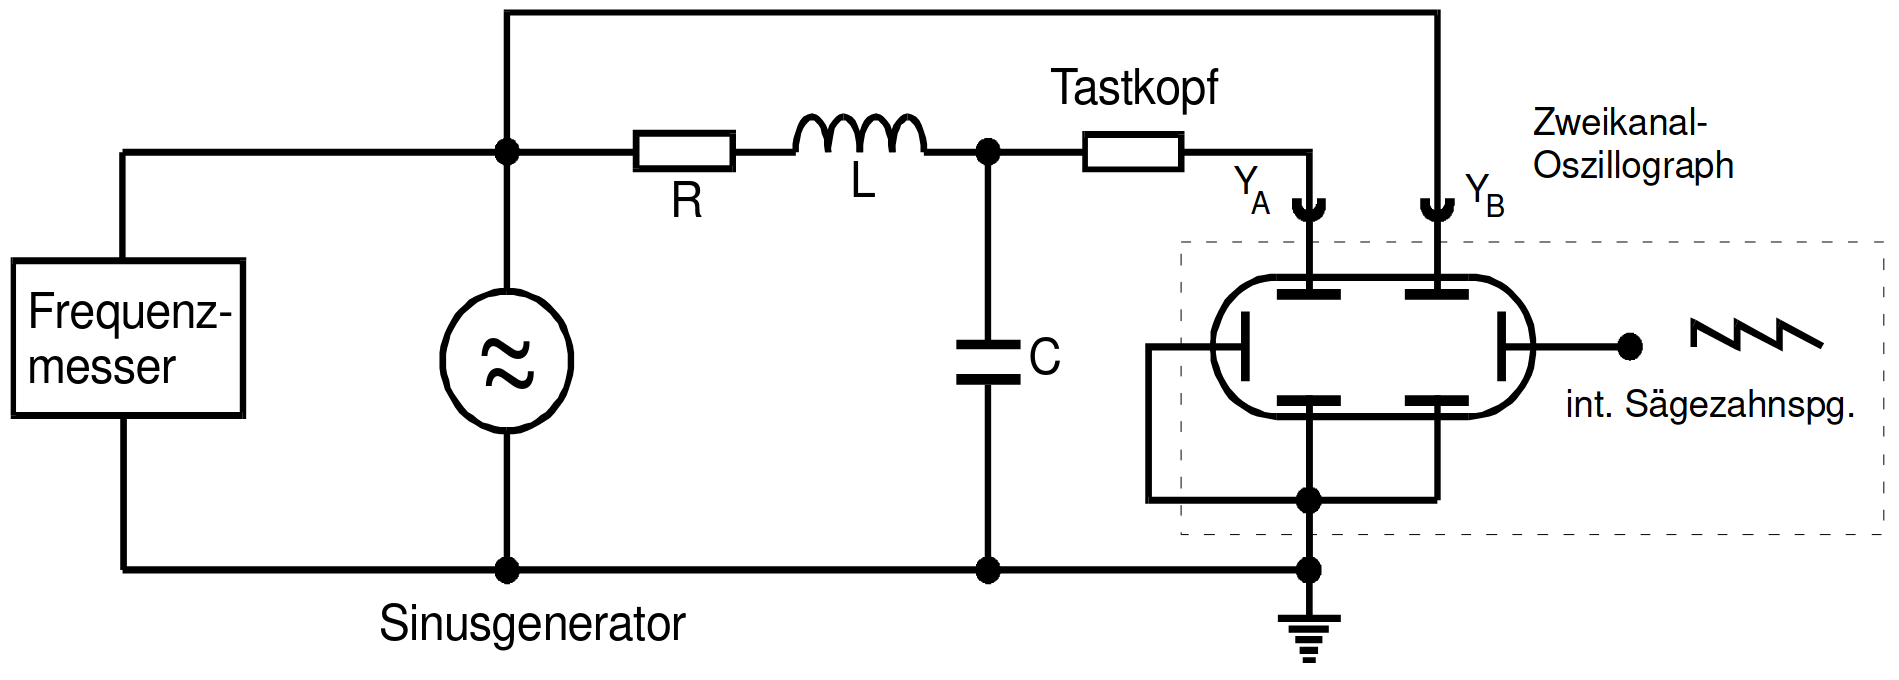
\includegraphics[width=\linewidth]{build/Kreis2.png}
    \caption{Schematischer Aufbau des dritten Versuchteils.\cite{V354}}
    \label{fig:Aufbau2}
\end{figure*}
\\
Im dritten Aufgabenteil wird die Frequenzabhängigkeit der Pase und der Kondensatorspannung gemessen.
Es wird wieder ein konstanter Widerstand mit $R = \SI{682(0.5)}{\ohm}$ eingebaut. 
Die Frequenz wird von $\SI{5}{\kilo\hertz}$ bis $\SI{70}{\kilo\hertz}$ erhöht. Es werden Werte für die Kondensatorspannung $U_C,$ die Erregerfrequenz $f,$ der Abstand $a$ der Nulldurch von $U_C$ und $U_0,$ sowie die Intervalllänge $b$ aufgenommen.\\
\\